\IEEEPARstart{E}{ste} trabajo se concentra principalmente en el an\'alisis
de las rutas que siguen los paquetes IPs enviados en una red hasta llegar a
su destino. Como se sabe, el protocolo IP (al ser un servicio no orientado
a conexi\'on), no nos asegura el orden ni el camino\footnote{Enti\'endase
por camino a los sucesivos saltos o \textit{hops}\cite{hop} los cuales
atraviesa un paquete IP para llegar a su destino.} que seguri\'a un paquete,
y es justamente el objetivo de este trabajo es poder observar dichos caminos:
como var\'ian, sus tiempos de respuestas, ubicaci\'on geogr\'afica, etc.

\par As\'i pues, podemos clasificar los pasos de este trabjo en 3 partes
bien definidas:
\begin{enumerate*}[label=\itshape\alph*\upshape)]
    \item el desarrollo de una herramienta que nos permita determinar el
        camino que siguen los paquetes IP hasta llegar a su destino y la
        informaci\'on asociada a cada camino que ser\'a luego analizada, 

    \item una experimentaci\'on variada con dicha herramienta para reunir
        informaci\'on, y

    \item un an\'alisis de la informaci\'on que nos permita llegar conclusiones
        sobre las capacidades y caracter\'isticas de los caminos que siguen
        los paquetes en la red global
\end{enumerate*}.

%-------------------------------------------------------------------------------

\subsection*{Notaci\'on}\label{sec:notacion}
\par A lo largo de este trabajo se utilizar\'a cierta terminolog\'ia que,
en el marco de la materia, puede ser interpretado de diferentes maneras. Por
ello que se presenta a continaci\'on un peque\~no glosario con los
terminos que utilizaremos de aqu\'i en m\'as y sus significados:

\bigskip

\begin{description}
	\item[Host] Representa las PC/Servidores (nodos de la red) en los
		extremos del experimento. En particular tendremos el 
		$host$ origen (las computadoras desde donde se realizaron
		los experimentos) y destino (las universidades seleccionadas).
	\bigskip

	\item[Hop] Hace referencia a todos los nodos intermedios ($routers$,
		$gateways$) que se encuentran entre nosotros y el host
		destino. En algunos casos, por abuso de notaci\'on, nos
		referiremos como $hop$ a alg\'un $host$ (de hecho, estos
		$hop$ tienen un sistema operativo\footnote{En muchos casos
		son servidores, o hasta posiblemente switches capa 3.}, por
		lo cual se podr\'ia decir que tambi\'en son hosts). El
		caso m\'as frecuente de esta utilizaci\'on del termino es
		cuando hacemos referencia al $host$ destino.
	\bigskip

	\item[RTT] $Round Trip Time$ entre el host de origen donde fueron
		corridos los experimentos y el $hop$ que respond\'io.
	\bigskip

	\item[RTT$_i$] Al agregar el sub\'indice al $keyword$ RTT,
		estamos hablando del RTT entre el i-\'esimo hops
		y su predecesor. Obviamente, por la naturaleza del experimento
		(con los TTL incrementales), dichos $RTT_i$ son la diferencia
		de los RTT muestrales entre los hops $i$ e \textit{i-1}.
	\bigskip

	\item[Ruta] Es una secuencia de hops que hay entre en host origen
		y el host destino. En algunos casos nos refer\'imos a esto
		como $path$ o $camino$.
	\bigskip
	
	\item[TTL] \textit{Time to Live}\cite{rfc792} de los paquetes $ICMP$
	\bigskip

	\item[TimeExceeded/EchoReply] Son posibles mensajes del protocolo $ICMP$%
	\cite{rfc792}. El primer ocurre cuando el TTL de un paquete llega
	con valor 1 a un hop, el cual descarta el paquete y env\'ia el mensaje
	$TimeExceeded$ a la IP de origen, para informar que su paquete fue
	descartado. El $EchoReply$ es la respuesta que da el host destino
	cuando recibe el paquete enviado.
\end{description}

%-------------------------------------------------------------------------------

\subsection*{Herramienta desarrollada: \textit{El Rastrearutas}\footnote{Se
pronuncia con acento espa\~nol.}}\label{sec:traceroute}
\par La herramienta adjunta a partir de la cual se reuni\'o la informaci\'on
analizada en este trabajo fue realizada siguiendo la metodolog\'ia propuesta
por el enunciado: enviar paquetes \textit{ICMP}\cite{rfc792} incrementando
su \textit{TTL} (comenzando desde 1) para luego recibir las respuestas de los
\textit{routers/swtiches} que conforman los hops del camino que sigue el paquete
enviado. Estas respuestas ser\'an del tipo \textit{TimeExceeded} hasta el
momento en que se alcance el \textit{host} destino, cu\'ando la respuesta ser\'a
\textit{EchoReply}

\begin{figure}[hbt]
	\centering
	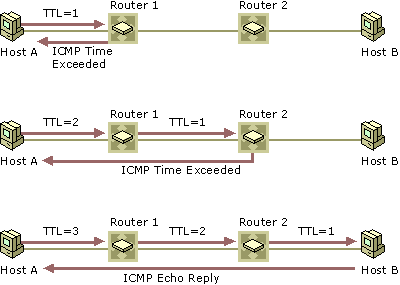
\includegraphics[width=0.5\textwidth,
			]{img/introduccion/rastrearutas.png}
	\caption{Metodolog\'ia TTL incrementales}
	\label{fig:metodologia_rastrearutas}
\end{figure}

\par Podr\'ia darse el caso en que no se alcance el
host destino. Esto podr\'ia deberse a m\'ultiples factores: el host destino
no responde los paquetes ICMP, alg\'un hop intermedio no \textit{fowardea}/%
delega este tipo de paquetes (para reducir su carga, por ejemplo), el host
se encuentra ca\'ido, congesti\'on de la red, e infinidad de motivos m\'as.

\par Nuestro trabajo consisti\'o en un primer lugar en desarrollar una
herramienta capaz de enviar estos paquetes ICMP siguiendo la metodolog\'ia
expuesta: modificando el campo TTL del \textit{header} IP y obteniendo la demora
entre el env\'io del paquete y su respuesta. Esto representa el \textit{Round
Trip Time} o RTT muestral obtenido\footnote{Este RTT es el tiempo transcurrido
entre el env\'io del paquete por nuestra herramienta y la respuesta obtenida.
M\'as adelante se calculara el RTT entre hops.}. Y este valor es tenido en
cuenta ya que luego ser\'a utilizado a la hora de analizar todos los datos
recibidos.

\par Esta herramienta fue desarrollada en \textit{python}\cite{python}
utilizando la librer\'ia/API \textit{scapy}\cite{scapy}, y todos sus resultados
fueron guardados un archivo de salida en formato \textit{csv}\cite{csv} para
luego ser analizados utilizando \textit{R}\cite{R}.

\par Vale la pena mencionar que por los motivos ya mencionados, podr\'ia pasar
que al enviar un paquete ICMP, este no obtenga respuesta (tanto el \textit{%
TimeExceeded} como el \textit{EchoReply}). Entre los motivos involucrados, bien
podr\'iamos encontrarnos con que un \textit{router} tuvo una sobrecarga
moment\'anea y tuvo que descartar paquetes, o motivos similares donde
normalmente obtendr\'iamos una respuesta. Para mitigar este tipo de situaciones,
nuestra herramienta fue hecha de manera tal que al no recibir una respuesta
luego de 1 segundo, considera que la respuesta no va a llegar (\textit{timeout})
y reintenta nuevamente con el mismo TTL. Luego de 3 intentos sin obtener una
respuesta, se considera que para dicho TTL no se puede obtener una respuesta
y se continua. El RTT calculado (entre el host origen y el host/router que nos
responde) no es acumulativo a trav\'es de los intentos. Es decir, una vez que
se lleg\'o al \textit{timeout} para un env\'io, no se considera el tiempo
transcurrido para calcular el RTT en el reintento siguiente.

%-------------------------------------------------------------------------------

\subsection*{Sobre los experimentos realizados}\label{sec:experimentacion}
\par Como se pide en el enunciado de este trabajo, se seleccionaron 3
universidades de distintos lugares del mundo para realizar la experimentaci\'on
y reunir la informaci\'on necesaria para cumplir con los objetivos propuestos.

\par A su vez, estas 3 universidades fueron seleccionadas teniendo en cuenta
los contintentes y las distancias desde donde se inician los paquetes IP que
se utilizaran para analizar la red. As\'i es que se buscaron universidades
lo suficientemente lejanas (en cuanto a distancia f\'isica) con la idea de que
la conectividad entre ellas
requeri\'a de varios enlaces intermedios/\textit{hops}, a partir de los cuales
podremos extraer la informaci\'on a analizar.

%-------------------------------------------------------------------------------

\subsection*{Sobre los Datos analizados}\label{sec:datos_analizados}

\subsubsection*{Rutas Experimentales vs Rutas Reales}
\par A la hora de analizar los datos obtenidos mediante la experimentaci\'on,
varias decisiones debieron ser tomadas. En primer lugar, el experimento consiste en
enviar paquetes ICMP incrementando su TTL, y presuponiendo que el host que
nos responde el paquete $i$ es justamente el hop anterior al host que nos
responde el paquete $i+$. Es decir, tratamos de descubrir el camino
que har\'an los paquetes que enviaremos al host destino, pero como ya
se ha mencionado, el protocolo IP no nos asegura que los paquetes vayan
a seguir el mismo camino para 2 paquetes distintos. As\'i pues, nuestro
experimento que nos otorga una serie de hops consecutivos podr\'ian, en la
realidad, no serlo.

\par Ilustraremos este concepto a continuaci\'on. Sean los hops $h_0..h_n$,
donde el sub\'indice nos indica el TTL inicial del paquete ICMP respondido por
el host/router del hop $h$. Suponemos tambi\'en que el router/host asociado al hop
$h_i$ est\'a actuando como un balanceador de carga entre 3 distintos
\textit{gateways}. En el caso de las respuestas recibidas desde los hops, el
camino que siguan para alcanzar a nuestro host \textit{source} es irrelevante
para el comportamiento que se est\'a explicando.

\begin{figure}[h]
    \centering
    \includegraphics[width=0.5\textwidth]{network_paths}
    \caption{Caminos supuestos}
    \label{fig:network_paths}
\end{figure}

\par Como se puede observar, este experimento nos podr\'ia dar una toplog\'ia
de hops bastante alejada de la realida. A\'un as\'i, esta es una limitaci\'on
que tendremos debido a la metodolog\'ia del \textit{rastrearutas} utilizando
paquetes ICMP. Esperamos mitigar esta posible situaci\'on realizando una
cantidad considerable de experimentos (y luego qued\'andonos con
las secuencias de hops m\'as frecuentes\footnote{Que esperamos que sean
significativamente m\'as frecuentes que el resto.}). Esto se debe a que suponemos
que los dispositivos que reconocemos como hops tambi\'en se encuentran
respondiendo \textit{requests} provenientes de la red, y esperamos encontrar
los hops m\'as frecuentes por salto, lo que ser\'a una posible aproximaci\'on
al camino real m\'as frecuente que realizan los paquetes.

%-----------------------------------

\subsubsection*{Hops sin respuesta}
\par Como ya se ha mencionado en esta secci\'on, ocurre frecuentemente que
varios hops en una ruta no env\'ian la respuesta $TimeExceeded$ cuando reciben
un paquete ICMP con TTL 1. Los posibles motivos de este comportamiento ya fueron
comentados en p\'arrafos anteriores, lo que importa definir ahora es que
se har\'a ante esta situaci\'on a la hora de analizar los datos.

\par A la hora de analizar estos datos no hay mucho que se pueda inferir. Con
esta herramienta no se puede saber cual de todos los motivos posibles (o cuales)
son los que ocurren. Entonces, si bien se decide mostrar gr\'aficamente a
los hops que no responden, a la hora de calcular los $RTT_i's$ hay que tomar
una decisi\'on.

\par Por un lado se puede calcular la diferencia entre los hops que lo rodean,
y luego dividir ese RTT calculado por 2, para repartir de forma equivalente el
RTT entre el hop que no respondi\'o y el posterior (que si lo hizo).

\par El problema de esta decisi\'on ser\'ia que, extendiendo a muchos hops consecutivos
que no respondan (en la realidad observamos hasta 4 hops consecutivos sin responder,
pero esto no es determinante), podr\'ia ocurrir que uno de esos 3 tenga una
latencia significativa, mientras que los otros 3 no. Entonces al repartir equitativamente
la latencia de todos juntos entre ellos igualar\'a sus $ZScores$, haciendo muy
d\'ificil distinguir cual de ellos es un enlace significativo y cual no.

\par Para mitigar esto tomamos otro camino: ignorar el hop que no respondi\'o a los ICMP, e
hacer como si el salto se diera entre los hops que lo rodean. De esta manera
estar\'iamos asign\'andole un $RTTi$ bastante mayor al
hop posterior, lo cual nos afectar\'ia el an\'alisis posterior para identificar
enlaces significativos, pero al menos podemos asegurar que entre esa serie de hops
hay una latencia/$RTT_i$ importante, y se podr\'a buscar herramientas para determinar
cual(es) de ellos son los enlances destacados.

\par Esto se debe extender a la situaci\'on donde varios hops consecutivos
no responden: 

\begin{itemize}
    \item Sean los $hop_i$ y $hop_j$ hops descubiertos mediante
    la experimentacion.
    \smallskip

    \item Sea una sucesi\'on de hops que no respondieron $hop_k$
    para $i < k <j,k\in[1,k_n]$
    \medskip

    \item Entonces $RTT_k = 0$ y $RTT_j = RTT_{hop_j} - RTT_{hop_i}$
\end{itemize}
%-----------------------------------

\subsubsection*{$RTT_i's$ Negativos}
\par La otra decisi\'on que debi\'o tomarse fue a la hora de calcular los $ZScore$.
Por todos los motivos que ya se explicaron, ocurre que muchas veces los RTT
de hops posteriores son menores que lo de hops anteriores. Si se analizan esos datos,
se analizar\'an $RTT_i's$ negativos, los cuales conceptualmente no tienen sentido, pues
no se puede \emph{ganar} tiempo en un salto\footnote{\url{http://www.imdb.com/title/tt0088763/}}.

\par As\'i pues, se decidi\'io, en primer lugar, no tomar en cuenta aquellos hops
que tuvieran un $RTT$ superior al del host destino o menores al del host origen. Luego,
al encontrarse saltos consecutivos entre los hops restantes que presentasen esta situaci\'on,
se decidi\'o descatar aquel hop con mayor desv\'io est\'andard, pues esto ser\'ia un
indicio de que dicho hop es un $outlier$ para el an\'alasis que se ha realizado.
